% !TEX root = ../thesis.tex
\documentclass[thesis.tex]{subfiles}
\begin{document}



\chapter{Background}
\label{chapter:background}

Tässä osassa selvitetään, mitä tutkimuksen kohteena olevasta aiheesta tiedetään entuudestaan. Selvityksen tulee kattaa tasapainoisesti koko tutkimuskenttä.

\section{Existing solutions}

There is a wide spectrum of technologies available for product authentication. Applications range from the use of inexpensive seals and electronic labels to carefully crafted watermarks and even DNA. These technologies can be categorized in many ways, for example, by their level of security, cost and portability. The focus of this chapter is on commercial smartphone-based product authentication technologies that often trade high precision (or reliability) for better cost-efficiency and portability. The technologies discussed can be considered as competing solutions for the technology developed in this thesis. Due to the nature of the topic the information on most of the technologies is limited in detail. An in-depth overview of product authentication technologies and their background is given in \cite{kuosmanen}.

\begin{figure}[ht]
\centering 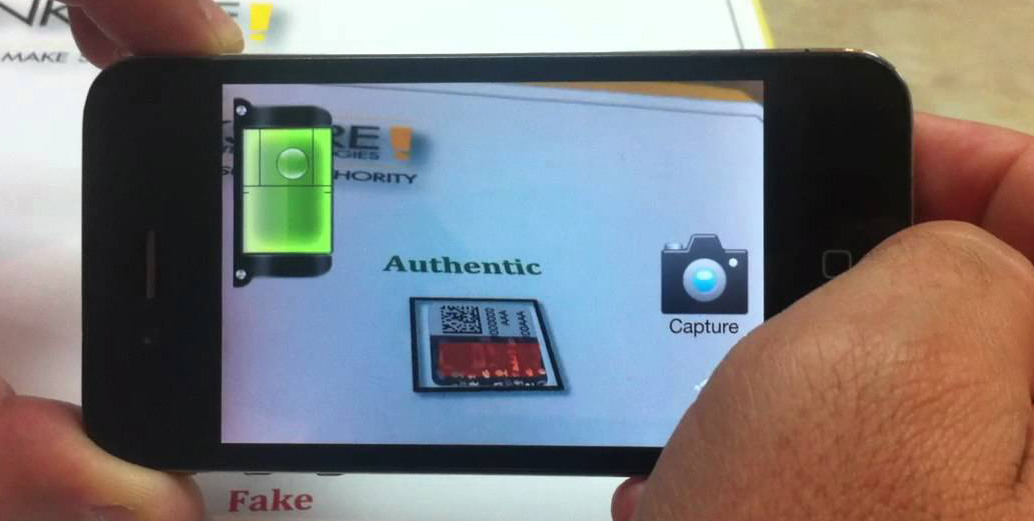
\includegraphics[width=13.25cm]{images/existing_solutions/smartsure}
\caption{InkSure's SmartSure iPhone application UI. The red rectangle and a virtual spirit level are used to position the smartphone correctly. \cite{inksure} \label{figure:inksure}}
\end{figure}

InkSure's SmartSure technology authenticates products by using a chemical marker (taggant) embedded into a hologram. Upon scanning the hologram, the application verifies it based on the presence of the taggant. The taggant is authenticated via a cloud-based platform that also offers track-and-trace reporting services. The application uses a QR scanner and visual aids to help the user position the smartphone's viewfinder properly over the hologram. \cite{inksure} An image of SmartSure's user interface can be seen in Figure \ref{figure:inksure}.

AlpVision offers a technology called CryptoGlyph\textregistered, which uses a pseudo-random pattern of tiny dots (40-80 microns) printed on the coating of the material to authenticate products. The color and size of the dots are customized based on the packaging color. The authenticity of the product is verified by matching the pattern on the product to one stored in a remote database. As of this writing AlpVision's iOS and Android applications are not publicly available in their respective application stores, but instead distributed as tailored applications \textit{``to meet the client's unique authentication needs''}. \cite{alpvision} Figure \ref{figure:alpvision} illustrates how differently sized and color dots affect their visibility and how they are applied to the coating of a material.

\begin{figure}[hb]
\centering 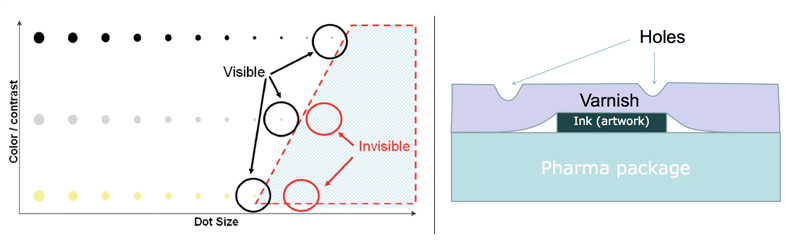
\includegraphics[width=13.25cm]{images/existing_solutions/cryptoglyph}
\caption{AlpVision's CryptoGlyph\textregistered{} embeds micro-dots on the coating of a material to create unique invisible patterns for product authentication \cite{alpvision}. \label{figure:alpvision}}
\end{figure}

The ever growing number of NFC-enabled phones (estimated to reach 53\% of the overall market in 2015 according to \cite{frost-sullivan}) has motivated companies to utilize NFC-based technologies for product authentication. Secure and specialized NFC tags have been manufactured by a number of companies since the technology first hit the market in 2006. However, only few companies have developed the software and services around NFC tags in order to provide end-to-end product authentication. A couple of active players in the field are FinnCode\footnote{\url{http://www.finncode.com/}} and Selinko\footnote{\url{http://selinko.com/}}, which both offer a SaaS-based solution for product authentication and manufacture secure NFC tags.

Other notable technologies built around the capabilities of a smartphone include scryptoTRACE\textregistered{} by U-NICA\footnote{\url{http://www.u-nica.com/1320.html}}, CertiEye by Infotoo Ltd.\footnote{\url{http://www.certieye.com/}} and AuthentiGuard by DSS Inc.\footnote{\url{http://www.authentiguard.com/products.html\#tab_authentiguard}}. A summary of the aforementioned technologies is provided in Table \ref{table:existing-solutions}. Next, Chapter \ref{section:photoluminescence} discusses photoluminescence and its applications.

\begin{table}[hb]
	\caption{Existing solutions for smartphone-based product authentication.} \label{table:existing-solutions}

	\begin{center}
	\begin{tabular}{| m{2cm} | m{3.25cm} | m{3cm} | m{3.75cm} |}

		\hline
		\textbf{Company}				&	\textbf{Product name}			&	\textbf{Platforms}			&	\textbf{Technologies} \\ \hline
		InkSure\newline (American)		&	SmartSure						&	iPhone						&	- chemical taggant\newline- hologram \\ \hline
		U-NICA\newline (Swiss)			&	scryptoTRACE\textregistered		&	iPhone, Android				&	- micro-printing\newline- edge detection \\ \hline
		AlpVision\newline (Swiss)		&	CryptoGlyph\textregistered		&	Customized\footnotesize{*}	&	- micro-printing\newline- pattern recognition \\ \hline
		DSS\newline (American)			&	AuthentiGuard					&	Customized\footnotesize{*}	&	 \\ \hline
		Infotoo\newline (Chinese)		&	CertiEye						&	iPhone, Android				&	 \\ \hline
		FinnCode\newline (Finnish)		&									&	iPhone, Android				&	- NFC \\ \hline
		Selinko\newline (Belgian)		&									&	Android						&	- NFC \\
		\hline
	\end{tabular}
	\end{center}
	\scriptsize{*} \small{privately distributed, the application is developed according to the client's needs.}
\end{table}

\section{Photoluminescence}
\label{section:photoluminescence}

Photoluminescence, one of the many forms of luminescence (light emission), is a process where a substance absorbs photons (light) and emits back a certain wavelength of light. Photoluminescence can be formally divided into two categories, \emph{fluorescence} and \emph{phosphorescence}, depending on the lifetime of the emission (decay time). Fluorescence typically occurs within a few nanoseconds whereas phosphorescence can last from a few milliseconds to seconds or even hours \cite{luminescence_basics}. Materials that have photoluminescent properties are typically referred to as luminophores (fluorophores and phosphors).

Figure \ref{figure:photoluminescence} illustrates the process of photoluminescence. Photoluminescence is initiated by \emph{photoexcitation}, the absorption of photons causing an electron to move to a higher energy state ($S_0 \rightarrow S_2$). The absorption is followed by internal conversion (IC), where the electron transitions within picoseconds from a higher to a lower energy state. After the electron has reached the lowest excited energy state ($S_1$) it relaxes to the ground state ($S_0$) and emits light (fluorescence), or an intersystem crossing occurs ($S_1 \rightarrow T_1$). The transition from the lowest triplet state to the ground state ($T_1 \rightarrow S_0$) eventually results to the emission of light (phosphorescence).

\begin{figure}[hb]
\centering 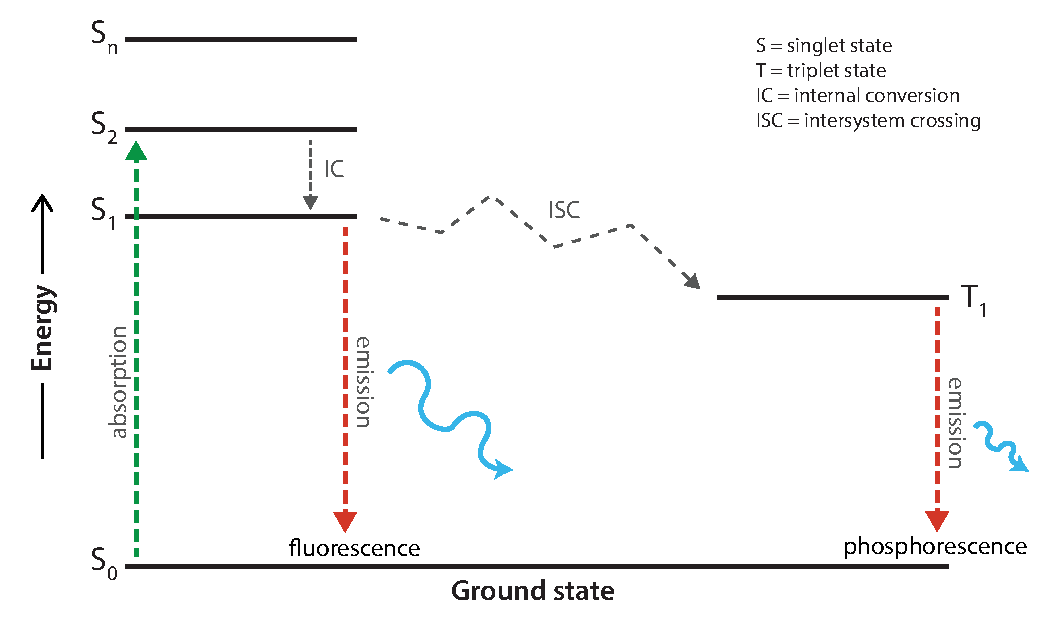
\includegraphics[width=13.25cm]{images/photoluminescence.pdf}
\caption{A simplified Jablonski diagram of photoluminescence. \label{figure:photoluminescence}}
\end{figure}

\noindent Since the energy of the electron at the triplet state is lower than at the singlet state phosphorescence occurs at longer wavelengths of light than fluorescence. Furthermore, the intersystem crossing from the singlet to the triplet state also alters the spin of the electron causing it to decay at a significantly slower pace. Thus, due to the longer excited state lifetime phosphors typically emit light long after the initial absorption of photons. \cite{CEJ}

Luminophores always emit longer wavelengths than they absorb. This is due to the loss of energy within the emission pathway. For example, during IC and ISC transitions some of the excitation energy gets transformed into heat. The difference between the absorption and emission wavelength is known as the Stokes shift. The magnitude of Stokes shift depends on the chemical properties of the luminophore. For fluorophores it is typically in the range of 30-50 nanometers while for phosphors, such as Lanthanide Chelates, it can range up to 200 nanometers. Luminophores are also subject to environmental effects \cite{hemmila}. Changes in temperature, pH, concentration or the amount of dissolved oxygen in the solution affect the intensity of the luminophore and can even shift its emission wavelength \cite{luminescence_basics}.

Photoluminescence can be used for detecting impurities \cite{photoluminescence_use_case_1}, tracing \cite{photoluminescence_use_case_2} and for studying the structure of a system \cite{photoluminescence_use_case_3}. The advantage of luminescence spectroscopy is that it allows analysing materials in a non-destructive and non-invasive manner. Commercially luminescence is used in illuminating watch faces under poor lighting conditions (Figure \ref{figure:photoluminescence_example}). The watch face gets illuminated when its phosphor-coated elements are excited by ionizing radiation. The radiation is induced by a radioactive substance enclosed in the phosphor coating. This form of luminescence is known as radioluminescence. Some less expensive watches use phosphorescence to achieve a similar effect: phosphors exposed to bright light continue glowing in the dark for a short time.

\begin{figure}[hb]
\centering 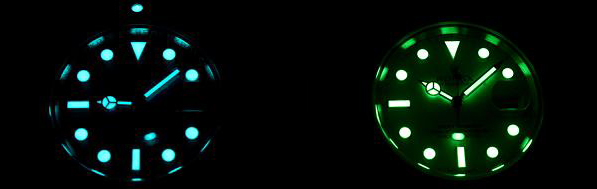
\includegraphics[width=10cm]{images/photoluminescence_example}
\caption{Watches use a radioactive substance (typically tritium) to illuminate their elements under poor lighting conditions.\label{figure:photoluminescence_example}}
\end{figure}

When a wavelength of light emitted by a luminophore falls in the visible spectrum of human eye (\mytilde390-700 nm) it creates a perception of a color. Color models are used to encode and represent this information in a medium. Chapter \ref{section:rgbhsv} provides an overview of three commonly used color models and their application areas.

\section{Color models}
\label{section:rgbhsv}

Color models provide an abstract mathematical model for describring colors numerically, typically as a vector of three or four dimensions. A color model alone is only sufficient for relative comparison of colors within that particular model. It is not until the model is given a \textit{context} that it forms a \textit{color space} and the relative colorimetric values get mapped to their absolute counterparts. Here context denotes a set of external (standardized) viewing conditions, in which the colors are expected to be rendered. For example, the standard sRGB color space is based on the RGB color model and assumes an ambient illuminance of 64 lux as per \cite{iec}. The term color model is sometimes referred to as \textit{non-absolute color space} or \textit{relative color space} even if it were less confusing to only speak about color models (relative) and color spaces (absolute).

The next sub-chapters provide a brief overview of a few widely adopted color models: RGB, HSV and YCbCr.

\subsection{RGB}
RGB is the most common color model found in today's computer displays and monitors. It is largely influenced by the historical research on human color vision: the Young–Helmholtz theory of trichromatic color vision, formulized in the 18th century, proposed that color vision is the result of three different photoreceptor cells (cone cells). Later, in 1956 this theory was backed by psychological evidence, which showed that the human retina is particularly sensitive to three groups of wavelengths in the areas of blue, green and red \cite{svaetichin}.

RGB is an \textit{additive} color model meaning that colors are produced by adding together two or more primary colors (red, green or blue). Adding all the primary colors together yields white. All RGB colors are defined relative to the primary colors, as the RGB color model itself does not specify what is meant by red, green and blue colorimetrically. For example, the color of pure yellow would contain all the red and green but no blue: RGB(100\%, 100\%, 0\%). The purpose of color spaces, such as sRGB, is to define the exact values (chromaticities) for the primaries, typically in terms of so called \textit{tristimulus values} (X, Y and Z). The tristimulus values map to a color in the \textit{CIE x-y chromaticity diagram}, which has been established through empirical research to represent all of the chromaticities visible to average human eye \cite{cie}. As seen in Figure \ref{figure:srgb}, a given color space can only produce the colors that fall within its \textit{gamut}, the triangle defined by the chromaticities of its primaries.

\begin{figure}[ht]
\centering 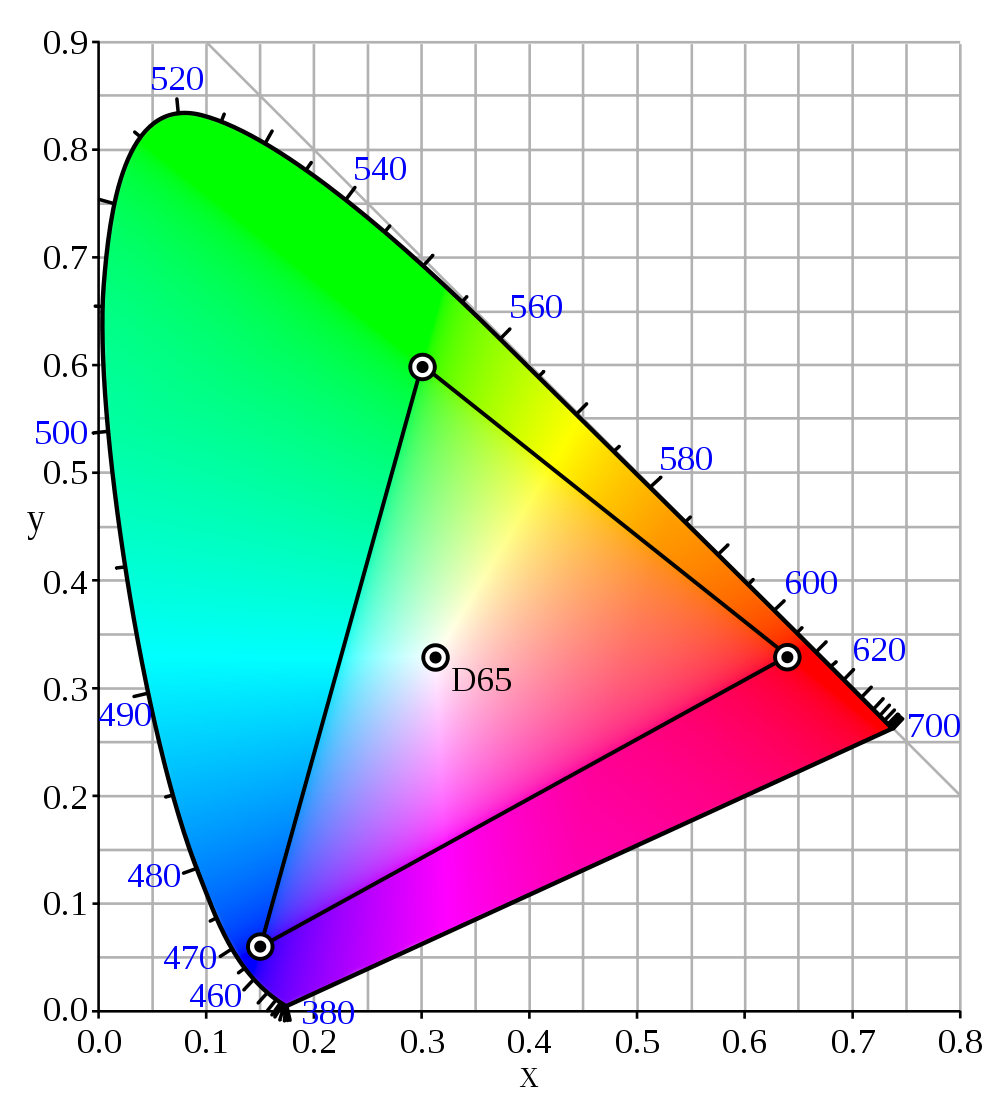
\includegraphics[width=10cm]{images/srgb}
\caption{The CIE x-y chromaticity diagram and sRGB gamut (triangle). A color space can only render the subset of colors that are within its gamut.\label{figure:srgb}}
\end{figure}

As evidenced by the wide adoptance of sRGB in digital consumer products, RGB is able to model the human color vision with reasonable accuracy. However, for some use cases there exists better alternatives as covered next in more detail.

\subsection{HSV}

HSV (hue-saturation-value) was developed in the late 1970s originally for computer graphics applications in an attempt to create a more intuitive and perceptually relevant color model. HSV rearranges the cartesian geometry of RGB to a cylindrical coordinate system separating the color information (chroma) from the brightness/intensity information (luma). These geometrical representations of RGB and HSV are depicted in Figure \ref{figure:rgb_hsv}. The ability to decouple luma from chroma brings many benefits in image processing applications. Many basic computer vision algorithms designed for grayscale images, such histogram equalization, canny edge detection or binary thresholding, become trivial in HSV space, since the processing can be done on the luma component (V) alone \cite{color_segmentation}. HSV is also the defacto choice for color pickers as hue, saturation and brightness are both conceptually and perceptually easier to reason about than red, green and blue.

\begin{figure}[ht]
\centering 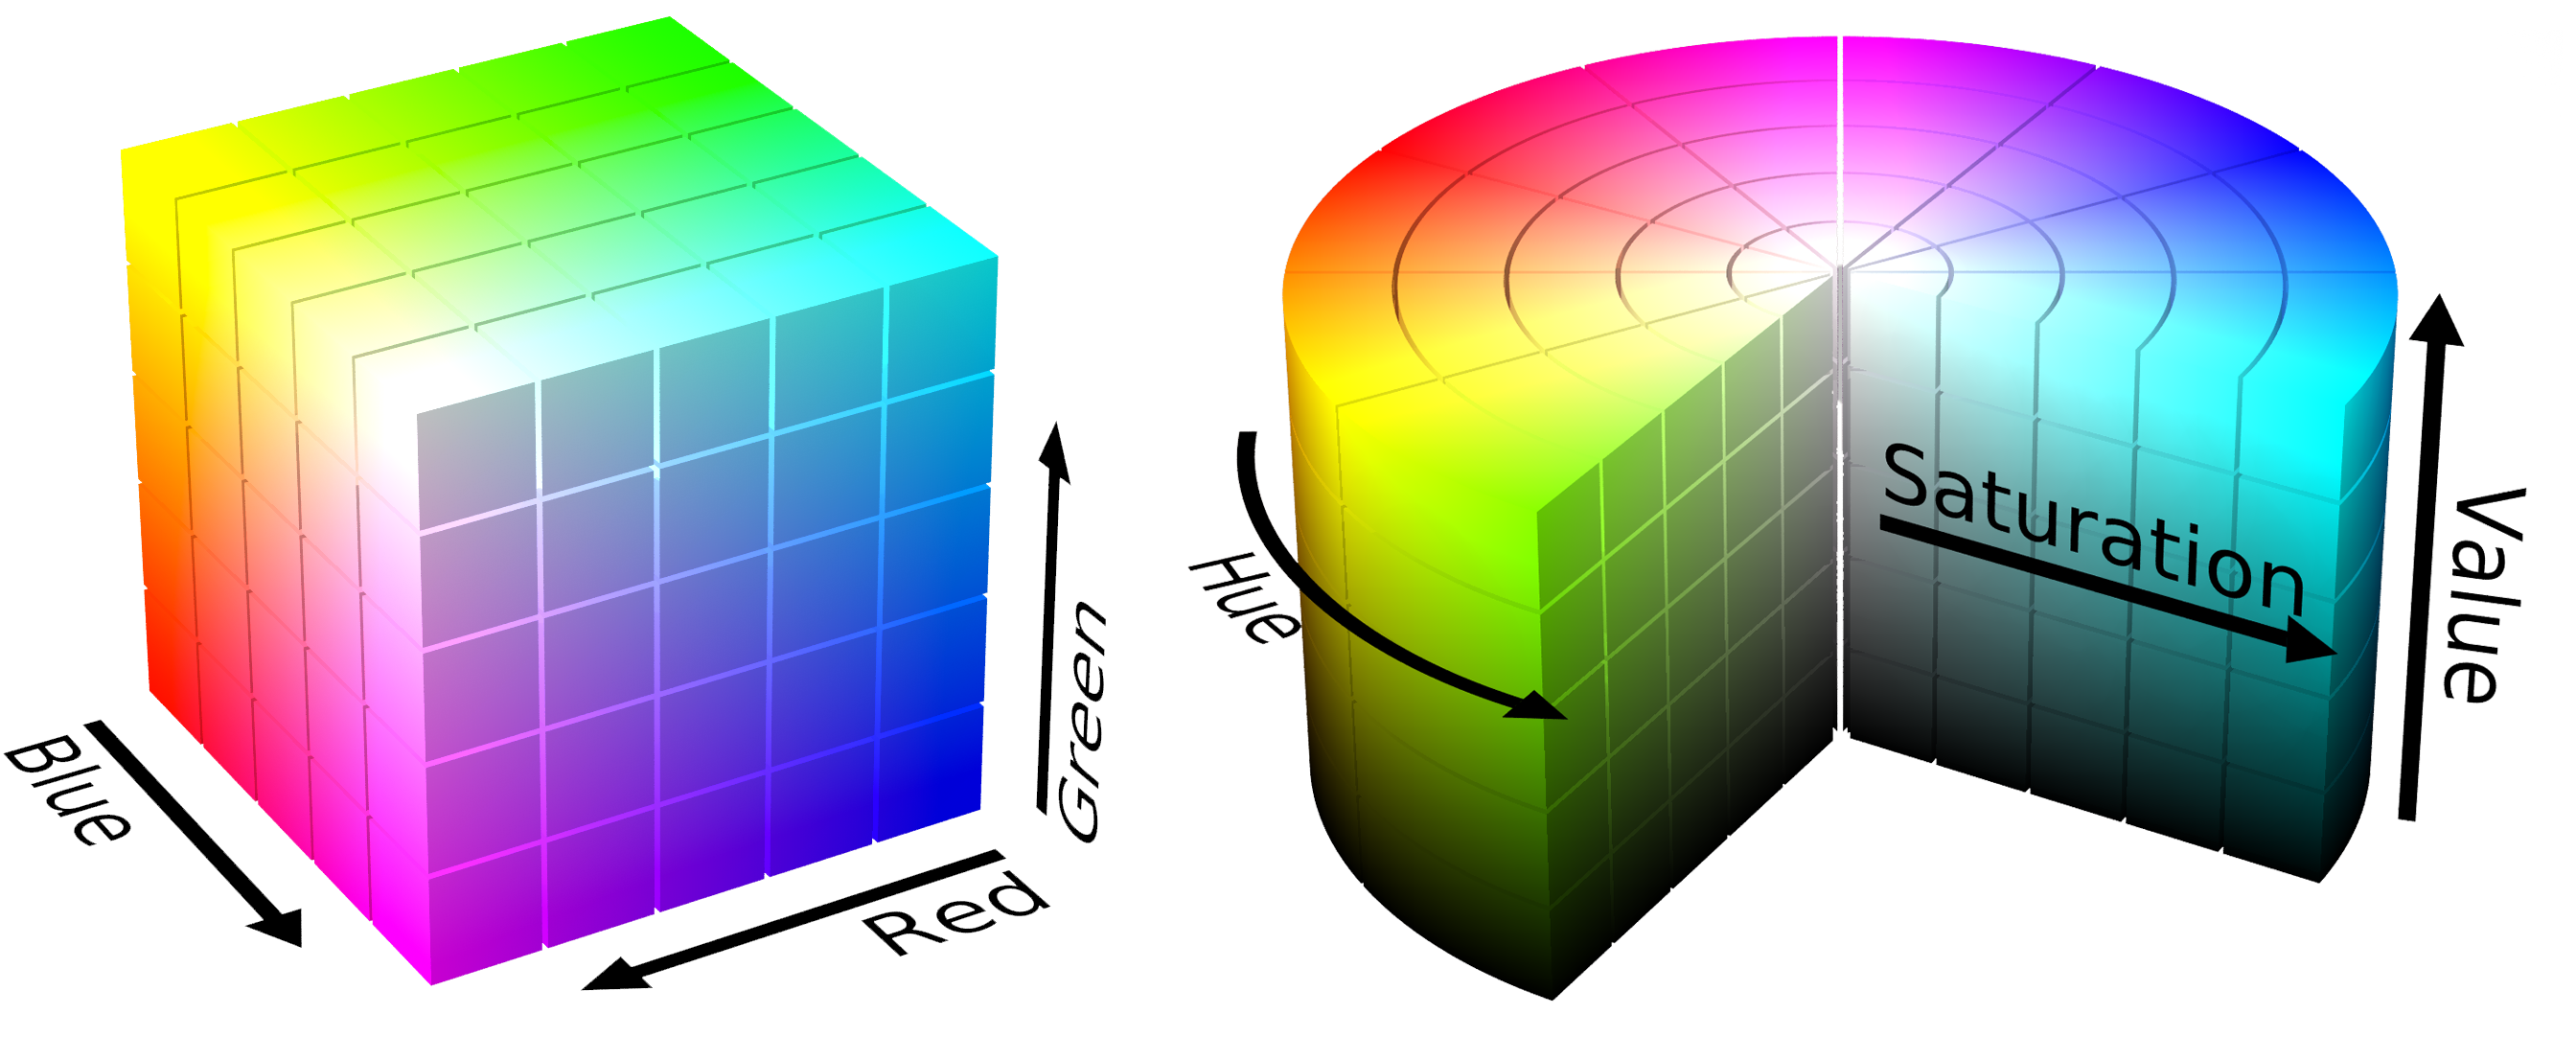
\includegraphics[width=13.25cm]{images/rgb_hsv}
\caption{RGB colors are typically displayed in cartesian coordinates, whereas HSV colors use cylinder coordinates \cite{hsv_cylinder} \cite{rgb_cube}.\label{figure:rgb_hsv}}
\end{figure}

RGB values can be converted into HSV using a simple linear transformation. The formal definition of the transformation can be given as follows:

\begin{align*}
C_{max}&=max(R, G, B),	&	C_{min}&=min(R, G, B),	&	C_{delta}&=C_{max}-C_{min}
\end{align*}
\begin{align*}
V &\leftarrow C_{max}	&
S &\leftarrow
	\begin{cases}
		\frac{C_{delta}}{C_{max}}, & \text{if $V\neq0$}\\
		0, & \text{otherwise}
	\end{cases}			&
H &\leftarrow
	\begin{cases}
		\frac{60(G-B)}{C_{delta}}, & \text{if $V=R$}\vspace{2mm}\\
		\frac{120+60(B-R)}{C_{delta}}, & \text{if $V=G$}\vspace{2mm}\\
		\frac{240+60(R-G)}{C_{delta}}, & \text{if $V=B$}
	\end{cases},
\end{align*}

\noindent where $R, G, B = \{\ x\ \vert\ x \in \mathbb R\ \wedge\ 0 \leq x \leq 1\ \}$.


\subsection{YCbCr}
YCbCr (or YCC) is a family of color spaces used as a part of the color image pipeline of video and digital imaging systems. YCbCr was primarily developed to enable a way of storing and transmitting color information with minimal redundancy. Much like HSV it separates luma (Y) from chroma (Cb and Cr) but also compresses the chroma components for improved storage and tranmission capabilities. Because the human visual system is has lower acuity (sensitivity) for color than luminance, the signal can be optimized by compressing the color components. At normal viewing distances this incurs no perceptible loss of quality. Each YCbCr format uses different subsampling scheme for the compression. The most common YCbCr subsampling (or chroma subsampling) ratios are 4:2:2, 4:1:1 and 4:2:0. The last two digits of the ratio denote how the compressed chrominance information is compressed and encoded as visualized in Figure \ref{figure:ycbcr}. For example, in the 4:2:0 format both the horizontal and vertical resolution of the Cb and Cr chroma components are halved and stored in adjacent columns.

\begin{figure}[ht]
\centering 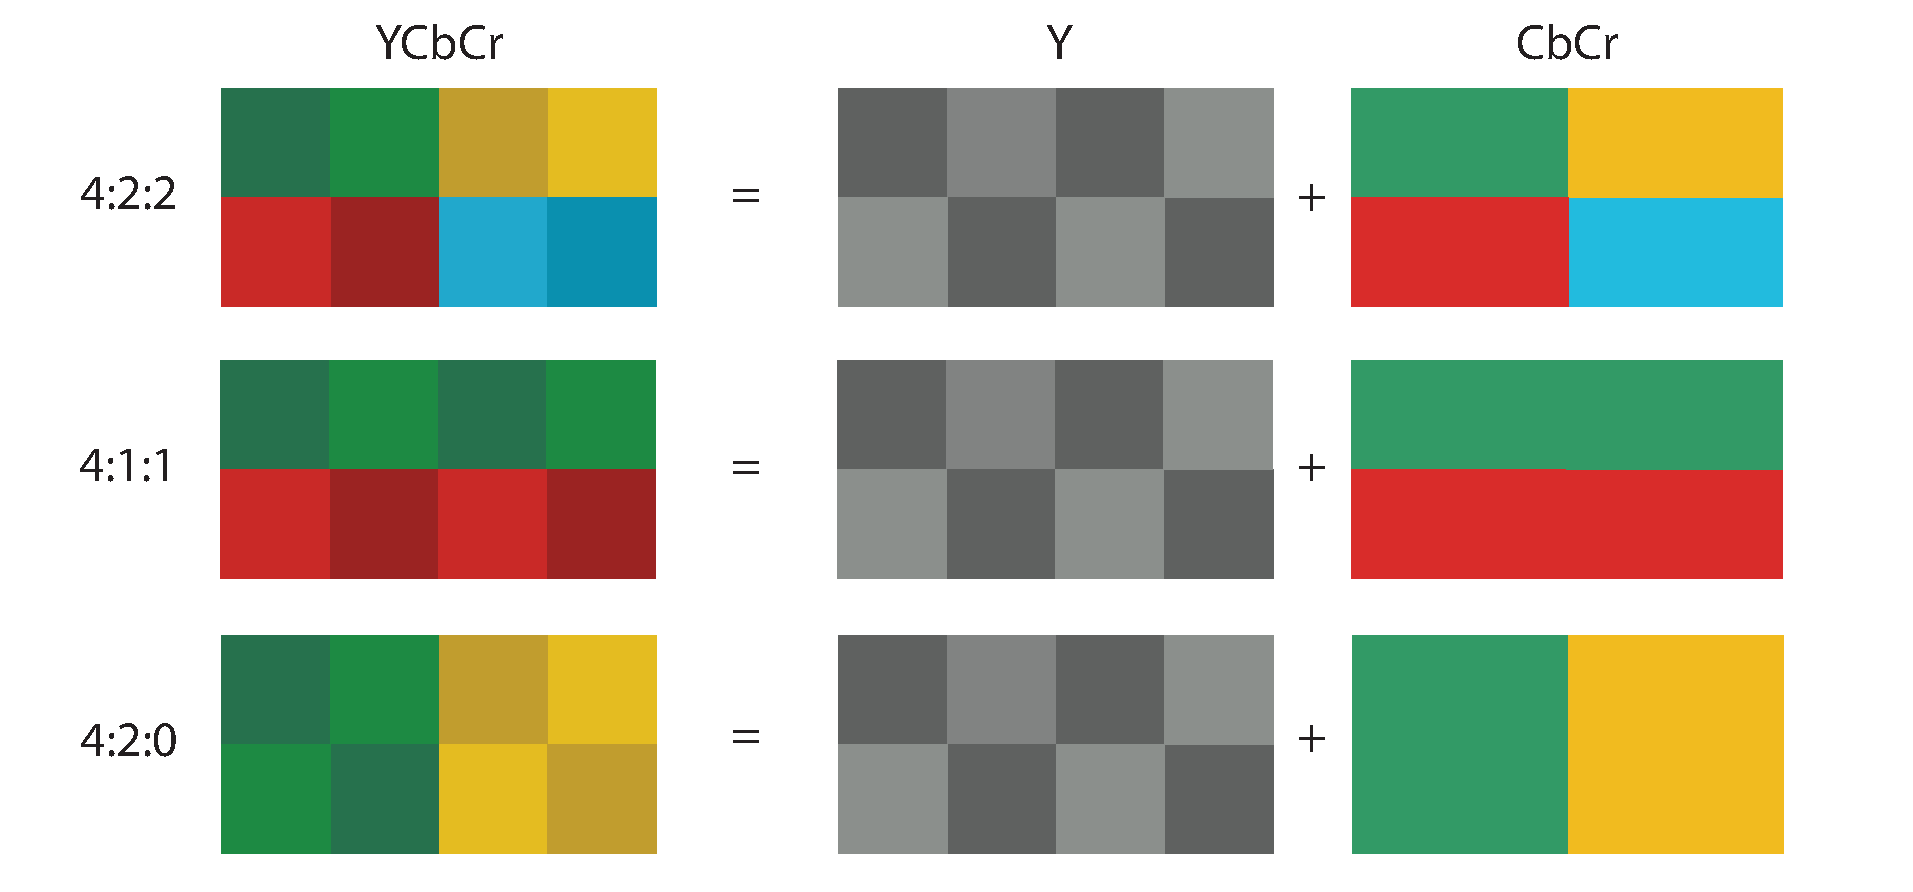
\includegraphics[width=13.25cm]{images/ycbcr}
\caption{ .\label{figure:ycbcr}}
\end{figure}


\section{Mobile Camera Technology}
device-dependency
\subsection{Sensors}
\subsection{Pixel Formats}
\subsection{Camera Flash}

\section{Hybrid Mobile Applications}
- jni, c++/cx, ios with c++?
- crosswalk project
- react native, reapp

Hybrid applications are essentially small websites running in a browser shell in an application that have access to the native platform layer. Hybrid applications have many benefits over pure native applications, specifically in terms of platform support, speed of development, and access to 3rd party code.

\end{document}